%!TEX root = report.tex
\exercise{Wavelet denoising}
\subsection{Wavelet denoising implementation}
One of the interesting applications of the wavelet transform is performing noise reduction on images. Noise can be introduced in an image in a variety of ways and can be aesthetically pleasing or even necessary to remove it from an image to make it useful. Wavelet-based noise reduction algorithms may be more useful than other algorithms when noise must be reduces while features must be preserved. As noise is mostly present in the details of the wavelet transform, the wavelet transform is a good candidate to apply noise reduction when features must be preserved.

Noise is usually removed in the wavelet domain by applying thresholding to the details. However, this can be done in two ways: one can either \textit{hard} or \textit{soft} filtering. In the case of hard filtering, if the absolute value of a pixel is below a threshold value the pixel is set to zero. However, this can lead to discontinuity in an image. The alternative is applying so called soft thresholding which involves hard filtering and then scaling the non-zero components towards zero. 

We have implemented both ways of scaling in the function \texttt{IPwaveletdenoise} which allows an user to threshold the $J$-scale wavelet domain of an image with either hard or soft filtering. The function is implemented as following:
\matlabexternal{../IPwaveletdenoise.m}

This function performs filtering in the details up to level $j$. The approximation is stored to restore it later on when the filtering is complete. In order to transfer it back to the spatial domain, the approximation is needed and would otherwise be lost in the filtering. 
The actual filtering is performed here:
\matlabexternal{../performFiltering.m}
The code performs exactly what it should do according to the description: it performs denoising by thresholding in the wavelet domain. 
\subsection{Denoising a noisy MRI image}
To ensure the code works we have executed the function on a noisy image in an attempt to denoise it. We have loaded \texttt{noisymri.tif}, which is a noisy MRI scan, in an attempt to denoise it. We have found out that a threshold value $t = 2$ is the best threshold value: it removes most of the noise while keeping most of the details. Figures~\ref{fig:noisyOrig} and~\ref{fig:noisyDenoise} illustrate the image before and after denoising with $t = 2$.
\begin{figure}[htb]
\centering
\begin{subfigure}{.5\textwidth}
  \centering
  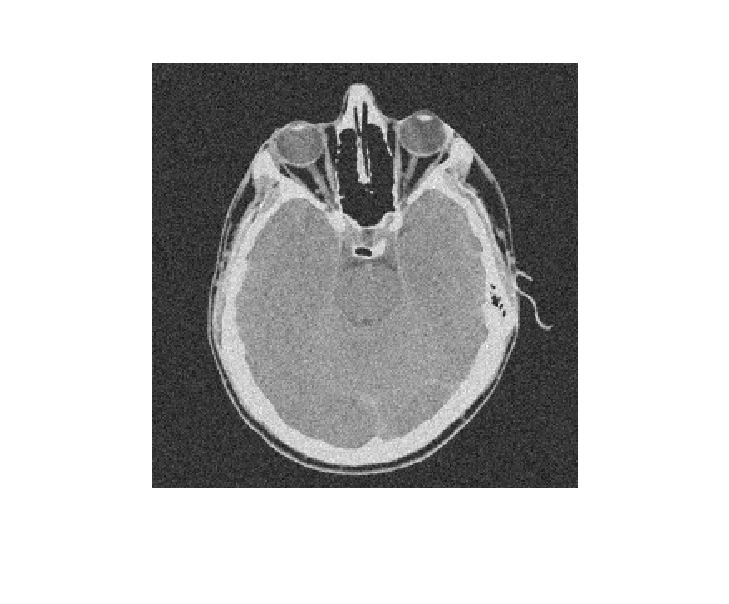
\includegraphics[scale=.7]{noisyMRI.eps}
  \caption{The original, noisy, MRI scan\newline}
  \label{fig:noisyOrig}
\end{subfigure}%
\centering
\begin{subfigure}{.5\textwidth}
  \centering
  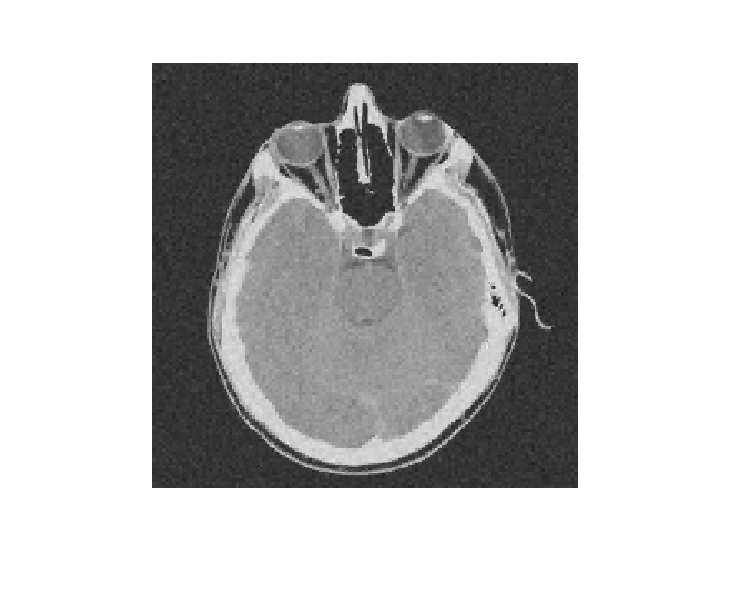
\includegraphics[scale=.7]{noisyMRI_Filtered.eps}
  \caption{The denoised image. Arguably, it is less noisy but the amount of detail is also lowered}
  \label{fig:noisyDenoise}
\end{subfigure}
\caption{An image of a MRI scan before and after denoising in the wavelet domain ($t = 3$, $j = 3$, $version = soft$)}
\label{fig:noiseReductionTest}
\end{figure}

Clearly, figure~\ref{fig:noisyDenoise} contains less noise than figure~\ref{fig:noisyOrig} while retaining most of its details. 
\clearpage